\subsection{Progettazione architetturale}
	\subsubsection{Prospetto orario}
	La distribuzione oraria della fase di Progettazione architetturale è la seguente:
\begin{table}[h!]
	\centering
	\renewcommand{\arraystretch}{2} 
	\rowcolors{2}{gray!25}{white}
	\begin{tabular}{|l c c c c c c|c| }
		\rowcolor{orange!50}
		\hline
		\multicolumn{8}{|c|}{\textbf{Suddivisione delle ore nei vari ruoli}}\\
		\hline
		\textbf{Nominativo} & RES 	& AMM 	& ANA 	& PRO 	& PRG 	& VER 	& \textbf{Totale} \\
		\hline
		\mat 				& - 	& -		& -		& 14	& -		& 10	& 24\\
		\hline
		\pie  				& -		& -		& 7		& -		& 7		& 10	& 24\\
		\hline
		\mic  				& 8		& 12	& -		& -		& 4		& -		& 24\\
		\hline
		\mar  				& -		& -		& 7		& 13	& 4		& -		& 24\\
		\hline
		\daG  				& -		& -		& -		& 14	& -		& 10	& 24\\
		\hline
		\daL  				& 8		& 12	& -		& -		& 4		& -		& 24\\
		\hline
		\gia  				& -		& -		& 6		& 7		& 11	& -		& 24\\
		\hline
	\end{tabular}
	\caption{Suddivisione ore del periodo di Progettazione architetturale}
\end{table}
Di seguito rappresentata anche in un grafico:
\begin{figure}[h!]
	\centering
	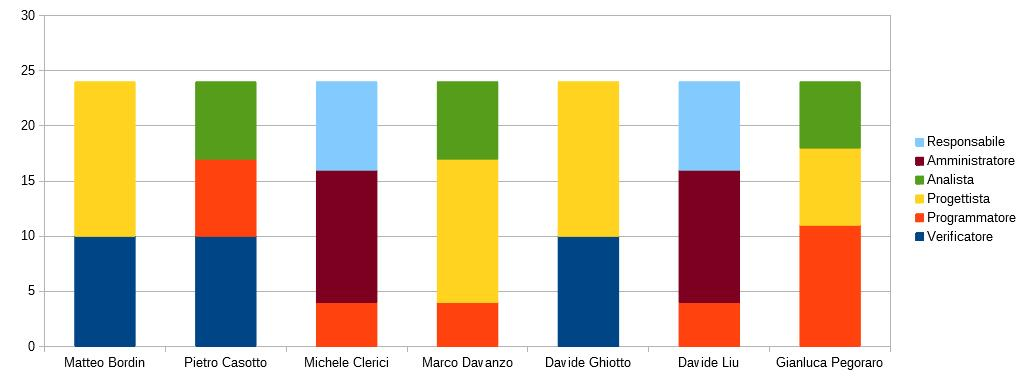
\includegraphics[width=\textwidth]{preventivo/grafico_seconda_parte.jpg}
	\caption{Grafico suddivisione oraria nel periodo di Progettazione architetturale}
\end{figure}

\subsubsection{Conteggio ore}
	La distribuzione delle ore nei vari ruoli nella fase di Progettazione architetturale è la seguente:
	
\begin{table}[h!]
	\centering
	\renewcommand{\arraystretch}{2} 
	\rowcolors{2}{gray!25}{white}
	\begin{tabular}{| c c c|}
		\rowcolor{orange!50}
		\hline
		\multicolumn{3}{|c|}{\textbf{Suddivisione ruoli in ore}}\\
		\hline
		\textbf{Ruolo} 			& Ore 	& Costo\\
		\hline
		\textbf{Responsabile}	&16		&480\\
		\hline
		\textbf{Amministratore}	&24		&480\\
		\hline
		\textbf{Analista}		&20		&500\\
		\hline
		\textbf{Progettista}	&48		&1056\\
		\hline
		\textbf{Programmatore}	&30		&450\\
		\hline
		\textbf{Verificatore} 	&30		&450\\
		\hline
		\textbf{Totale} 		&168	&3416\\
		\hline 
	\end{tabular}
	\caption{Ore e costi totali del periodo di Progettazione architetturale}
\end{table}
	~\newline Di seguito rappresentata anche in un grafico:
\begin{figure}[h!]
	\centering
	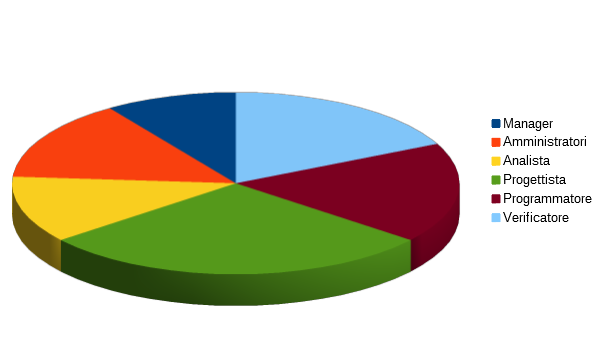
\includegraphics[scale=0.8]{preventivo/torta_seconda_parte.png}
	\caption{Grafico suddivisione ruoli nel periodo di Progettazione architetturale}
\end{figure}
\clearpage